
\section{Calorimetry}
\subsection{Calorimeters}

%%%%%% SLIDE
\begin{frame}{\textcolor{Goldenrod}{Calorimeter}}
  \(
  \<{0.54\textwidth}
  \img{36_CAL_shape.pdf}\\
  {\scriptsize Uranium/liquid-Argon (ULA) detector incorporating
    both EMCAL and HCAL over the full
    solid angle}
  \>
  \<{0.6\textwidth}
  \itt
\item[$\Box$] \hlt{black}{Design considerations:} \\
  \itt
\item[$1)$] good energy resolution
\item[$2)$] good electron ID close to other particles $\to$ fine
  transverse segmentation
\item[$3)$] good $\pi^{\pm}/e$ and $\gamma/e$ separation $\to$ fine
  longitudinal segmentation
  \tti
  % \item CC covers $|\eta | < 1$  and the two EC cover $|\eta | < 4$.

\item three liquid argon cryostats($ 90 K $): one central,  
  and two forward backward endcaps (coverage up to $|\eta | \approx 4$) 
  \tti
  \>
  \)
\end{frame}

%%%%%% SLIDE
\begin{frame}{\textcolor{Goldenrod}{Calorimeter's Unit Cell}}
  \(
  \<{0.7\textwidth}
  \itt[<+->]
\note{As an incoming particle interacts with the dense matter in the
  absorber plate, a shower of secondary particles is produced $\to$
  ionize argon atoms, and negative charge will drift towards the signal
  boards.}
  
\item signal is proportional to the energy loss of the incoming
  particle.
  
\item An insulating layer separates the pads from the outer surface. The
  resistive coating held at positive high voltage.

  \note{This method of
    readout has the advantages of keeping the pads away from ground to
    reduce noise, and eliminating blocking capacitors in the liquid
    volume.}
  
\item several unit cells stacked on top of each other are read out
  together ($\approx 47000$ channels).
\item
  Uranium has an appreciable advantage over iron:\\
  1) much better energy resolution for hadrons and
  jets\\
  2) the short absorption length
  \note{results in
    reduced shower size and thus permits the use of smaller towers.}
  \tti
  \>
  \<{0.4\textwidth}
  \img{37_CAL_unit_Cell}\\
  {\scriptsize an absorber plate $(U, Cu or Fe)$ followed by a gap filled with
    liquid argon and a $G-10$ board, with a $ \Delta V = 2.0 kV$ at the
    middle}
  \>
  \)
\end{frame}


%%%%%% SLIDE
\begin{frame}{\textcolor{Goldenrod}{Central Calorimeter}}
  \begin{overlayarea}{\textwidth}{\textheight}
    \begin{figure}[h]
      \centering
      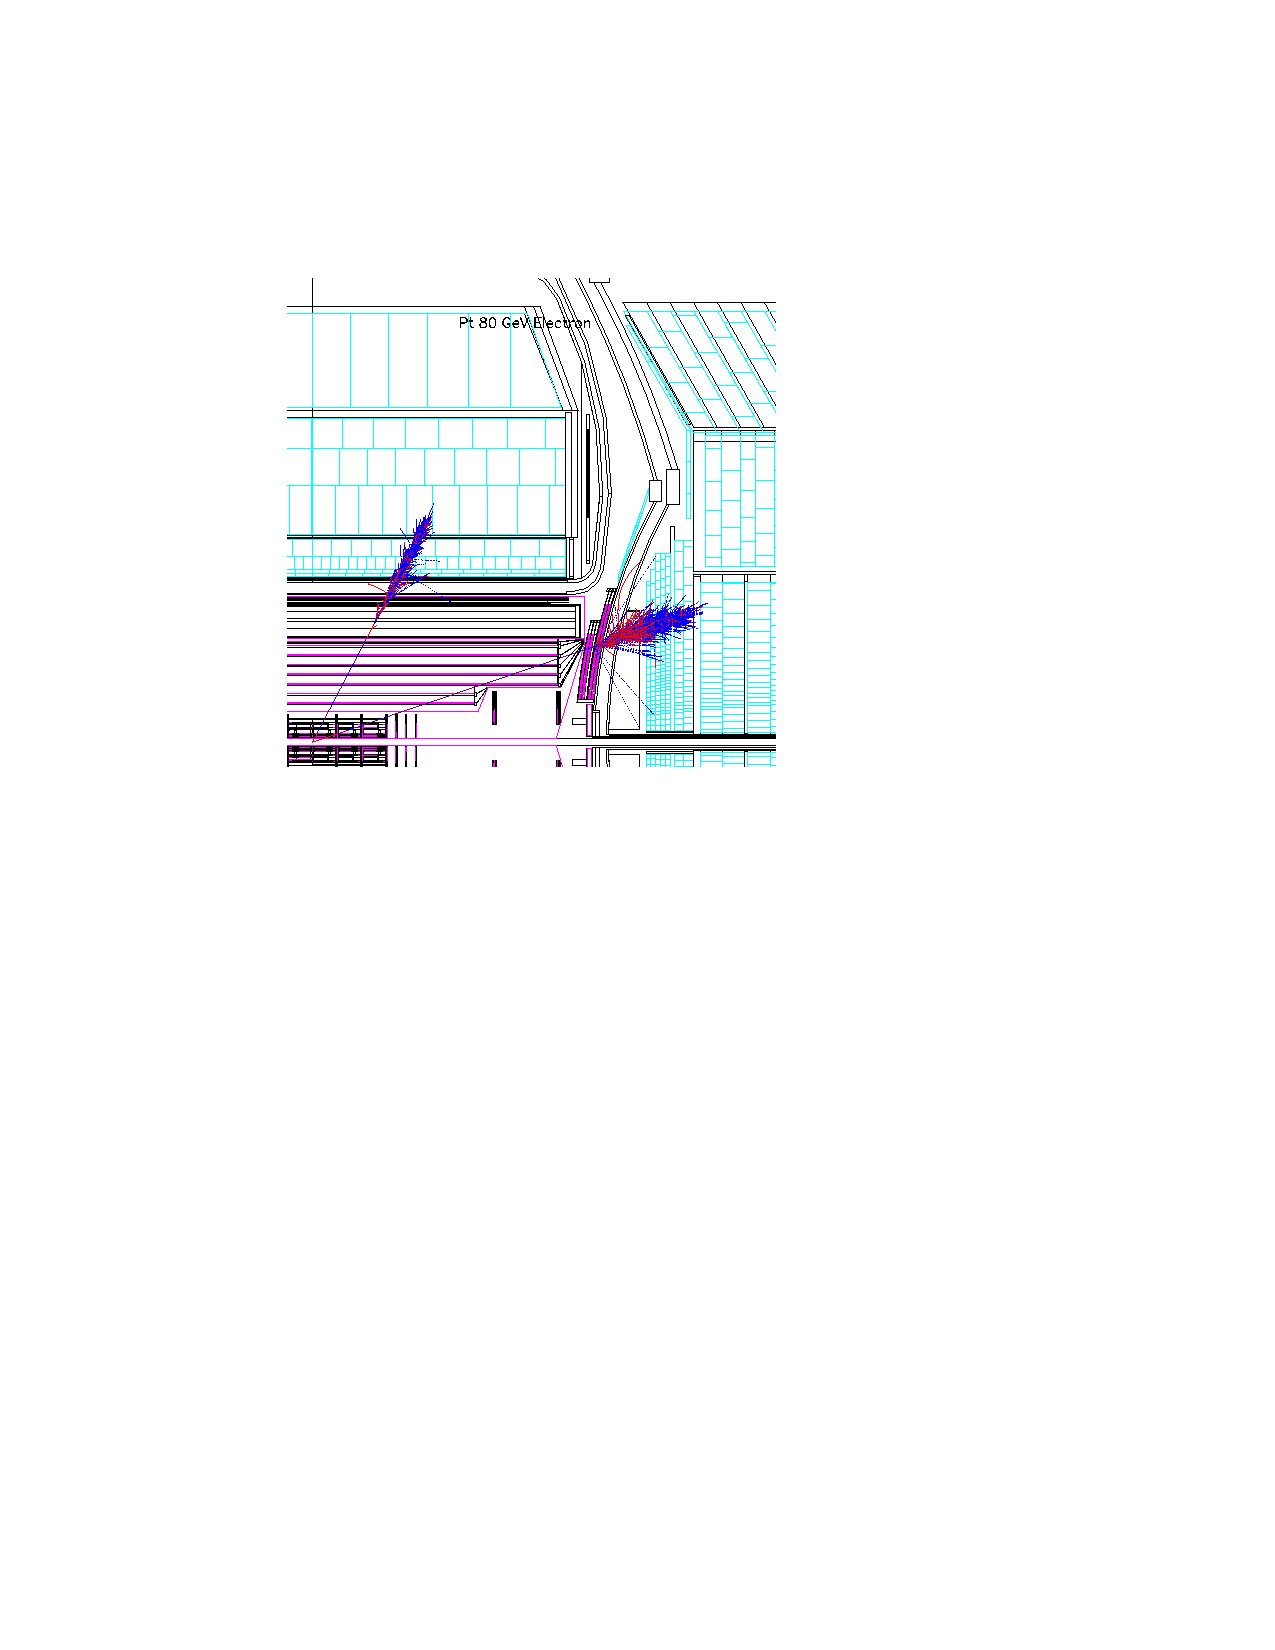
\includegraphics[height=0.4\textheight, width=0.6\textwidth]{./Images/40_CAL_showers.pdf}
      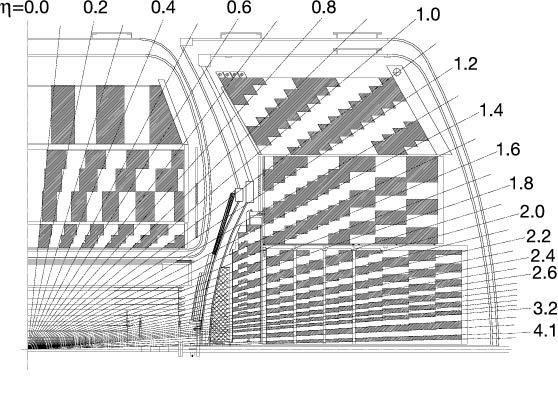
\includegraphics[height=0.4\textheight, width=0.45\textwidth]{./Images/38_CAL_central.jpg}
      
    \end{figure}

    \itt[<only@+>]
    \note{
      The shading pattern indicates groups of
      cells ganged together for signal readout.
      The rays indicate pseudorapidity intervals
      from the center of the detector.}
    
  \item[$\bullet$] multi-layer EM and hadronic modules:\\
    \begin{figure}[h]\centering
      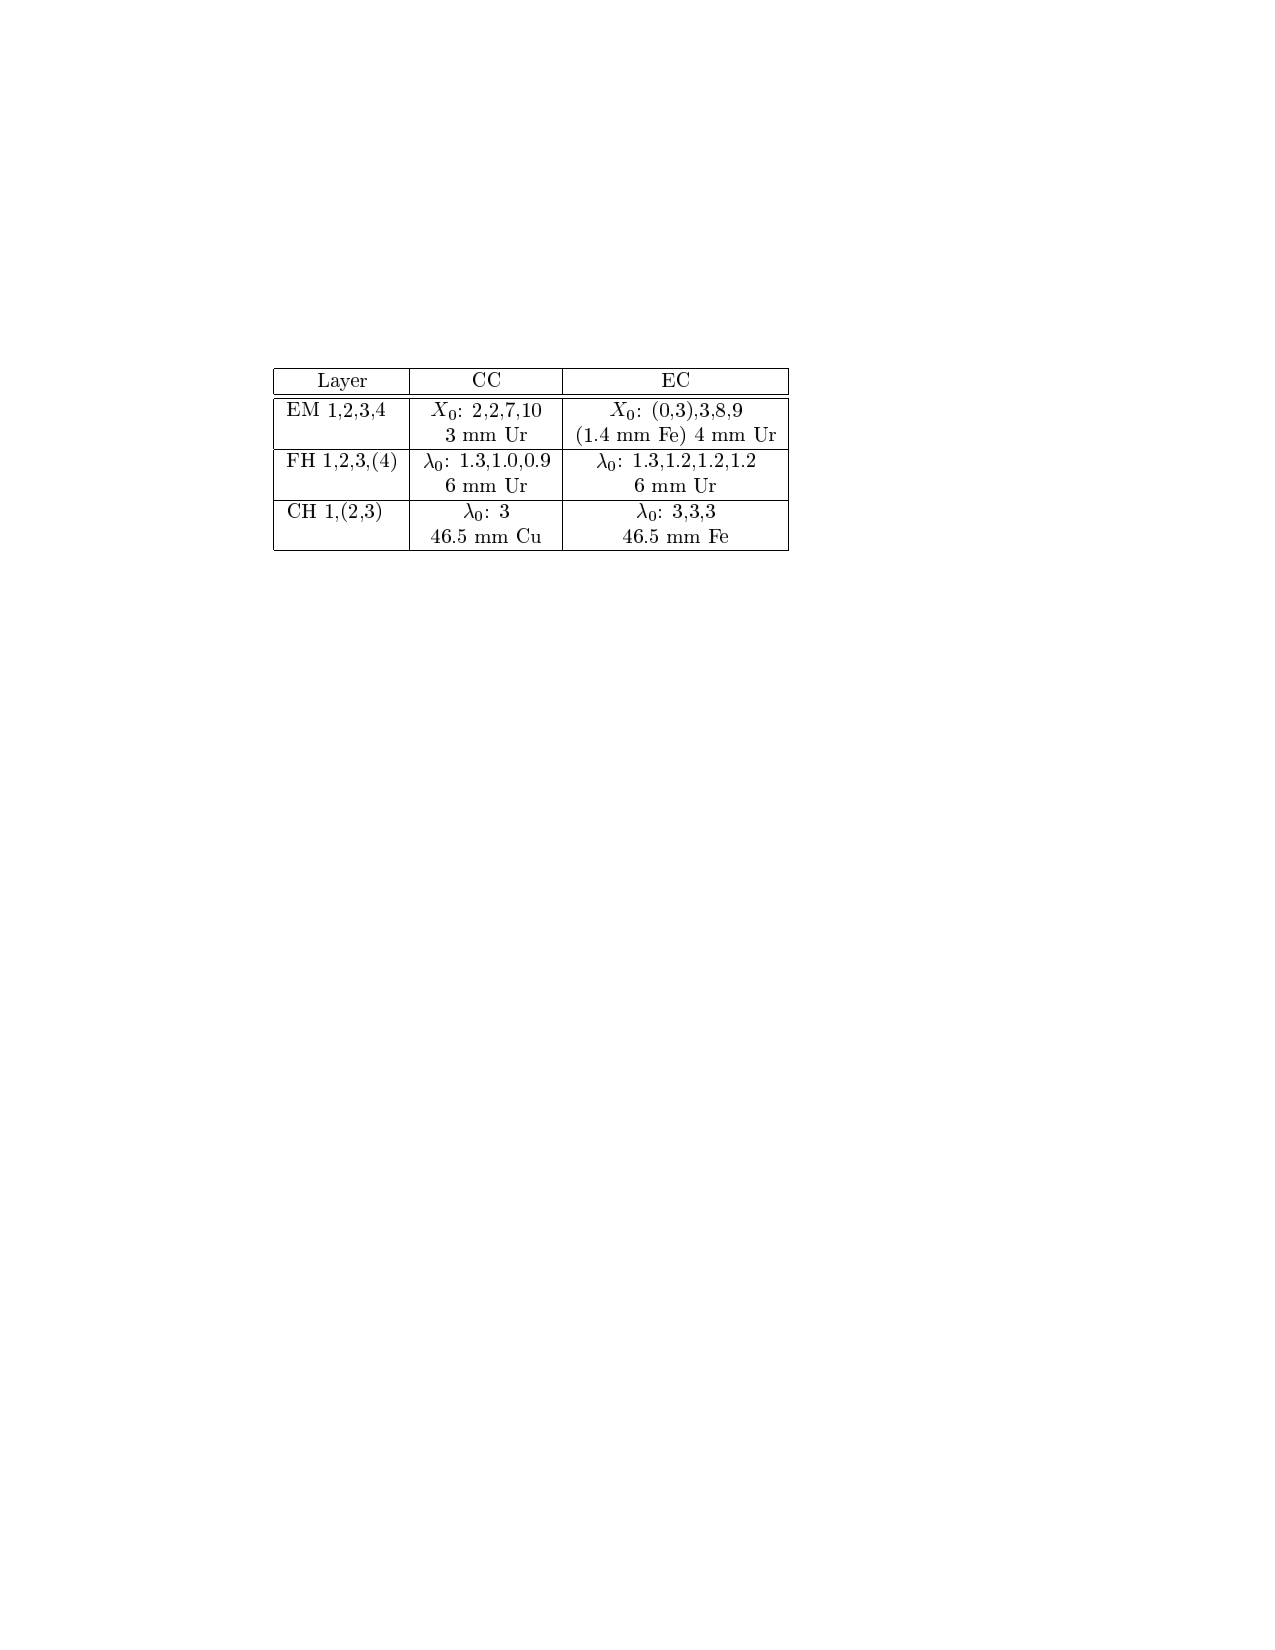
\includegraphics[height=0.2\textheight]{./Images/39_CAL_layers.pdf}
    \end{figure}
  \item[$\bullet$]
    The transverse sizes of the readout cells $\approx$ transverse sizes
    of showers: $1-2 cm$ for EM showers and about $10 cm$ for hadronic showers\\
    Towers in both EM and hadronic modules are $\delta \eta = 0.1$ and
    $\delta \phi \approx 5^{\textdegree}$
    
  % \item[$\bullet$]<1-> forward EMCAL is $24 X_0$ long with  $\delta E / E \approx
  %   0.10/\sqrt{E}$
    
  % \item[$\bullet$]<1->
  %   forward HCAL is $9 \lambda_0$ long  $\delta E / E \approx
  %   0.35/\sqrt{E}$
    
  \item[$\bullet$] dead region in between the three cryostats.\\
    $\circ$ a single layer array of $384$ scintillating tiles mounted on the
    face of both end cryostats.\\
    $\circ$ The scintillation light is taken by optical fibres to
    phototubes outside the magnetic field region.
    
    \note{The third layer of the EM modules, located at the EM shower maximum,
      is segmented twice as finely in both $\eta$ and $\phi$ to allow more precise location of
      EM shower centroids. Cell sizes increase in $\eta$
      and $\phi$at larger $\eta$ to avoid very small cells.}
    
    \tti
  \end{overlayarea}
\end{frame}

% %%%%%%% SLIDE
% \begin{frame}{\textcolor{Goldenrod}{Forward Calorimeters}}
%   \begin{overlayarea}{\textwidth}{\textheight}
%     \begin{figure}[h]
%       \centering
%       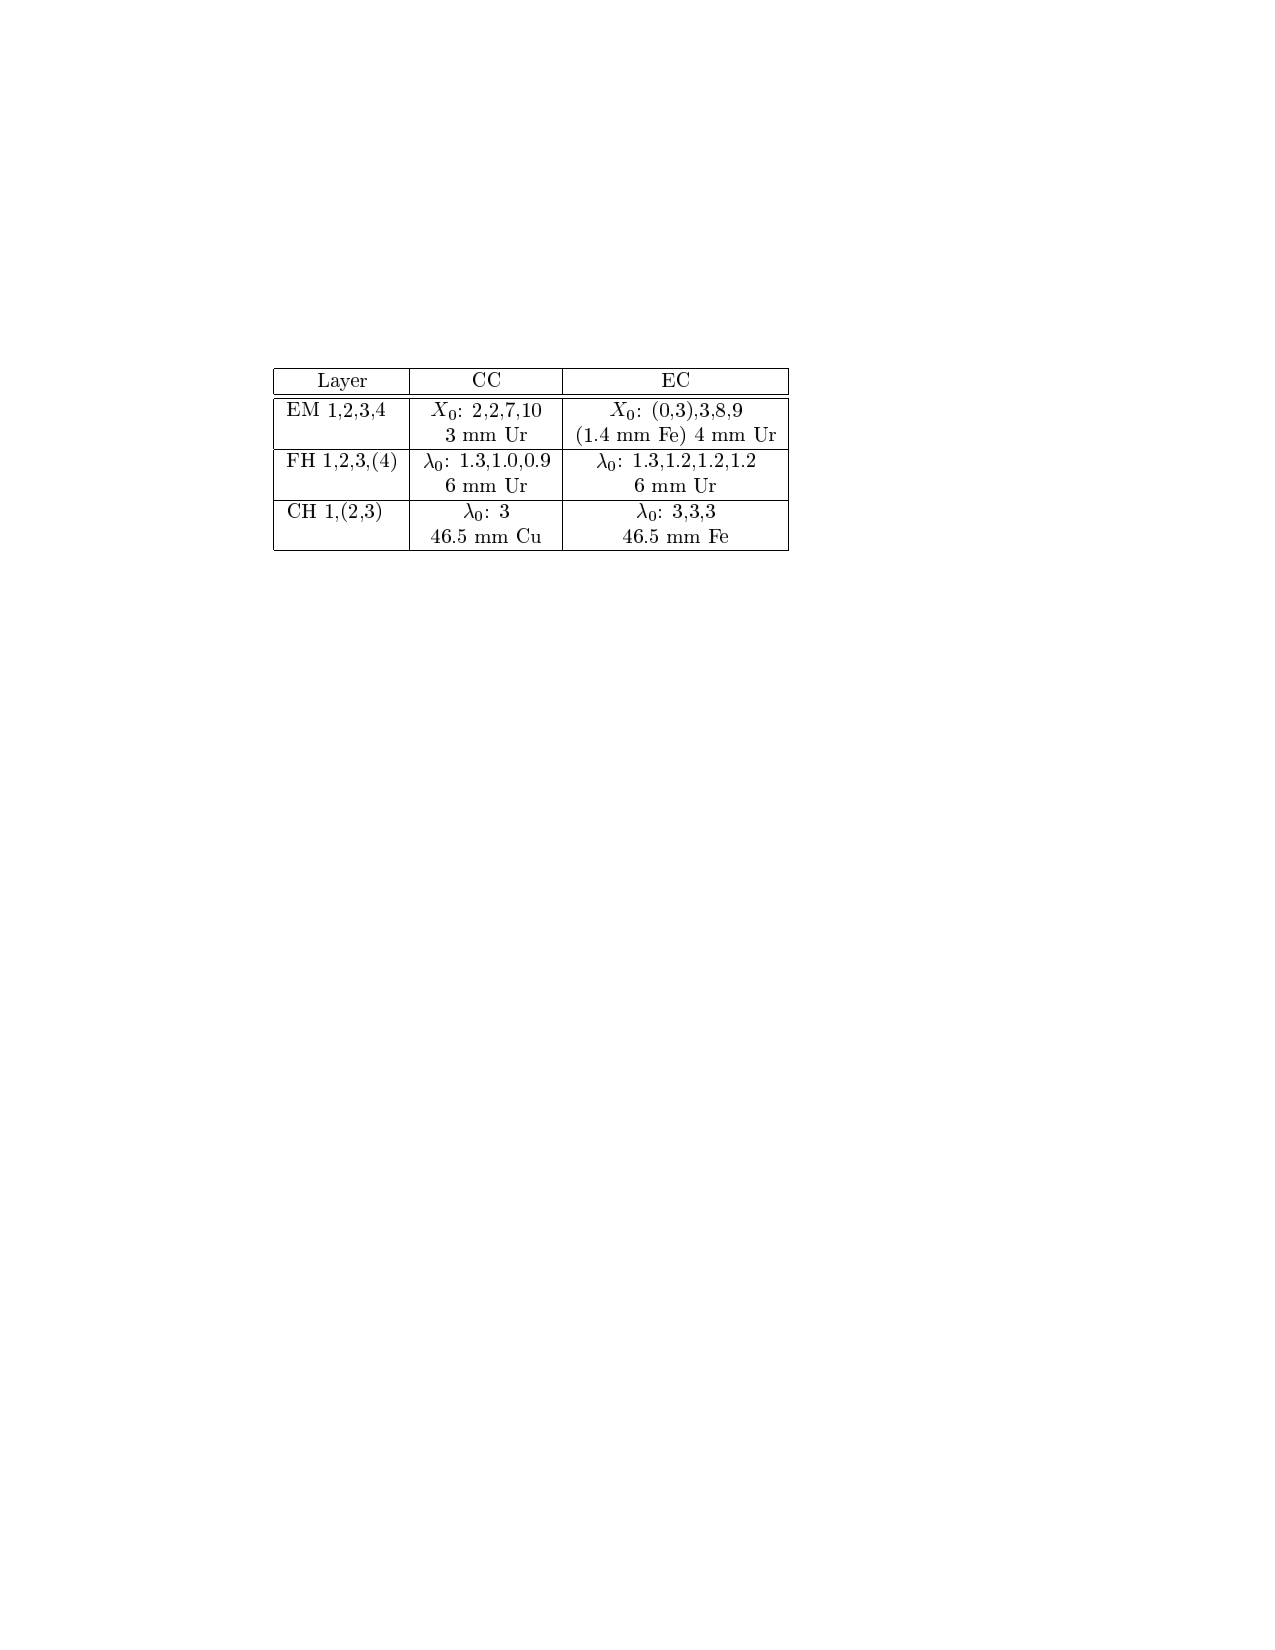
\includegraphics[height=0.3\textheight]{./Images/39_CAL_layers.pdf}
%     \end{figure}
    
%     \itt
%   \item[$\bullet$]<1-> forward EMCAL is $24 X_0$ long with  $\delta E / E \approx
%     0.10/\sqrt{E}$
    
%   \item[$\bullet$]<1->
%     forward HCAL is $9 \lambda_0$ long  $\delta E / E \approx
%     0.35/\sqrt{E}$
    
%   \item[$\bullet$]<2-> dead region in between the three cryostats.\\
%     \itt
%   \item a single layer array of $384$ scintillating tiles mounted on the
%     face of both end cryostats.
%   \item The scintillation light is taken by optical fibres to
%     phototubes outside the magnetic field region.
%     \tti
%     \tti
%     \note{
%       In the crossover region from the central to the end calorimeter, there
%       are several regions where particles travel mostly through support
%       structures (such as the cryostat walls).}
      
%       \note{To compensate for the energy
%         losses in these gaps there are extra sampling layers on the end faces
%         of the central calorimeter and on the inner faces of the end
%         cryostats, and there is also an intercryostat detector consisting of a
%         single layer array of 384 scintillating tiles mounted on the face of
%         both end cryostats. The tile size is chosen to match the calorimeter
%         cell size.}
      
%     \note{
%       There are three functionally distinct longitudinal sections for the
%       detector. The first is a very finely segmented EM calorimeter;
%       second is a less fine-grained hadronic section; and finally there is
%       a coarsely segmented hadronic "leakage" section.}

%   \end{overlayarea}
% \end{frame}  

%%%%%%%% SLIDE 
\begin{frame}{\textcolor{Goldenrod}{Central Calorimeter}}

  \itt[<+->]
  \item tt
  \tti
\end{frame}



%%%%%%%%% SLIDE
% \begin{frame}{\textcolor{Goldenrod}{Title }}
%   \begin{figure} \centering
%     %%%% figure manipulation 
%     \begin{tikzpicture}[zoomboxarray,connect zoomboxes, zoombox paths/.append style={ultra thick, red}]
%       \node [image node, help grid]
%       { 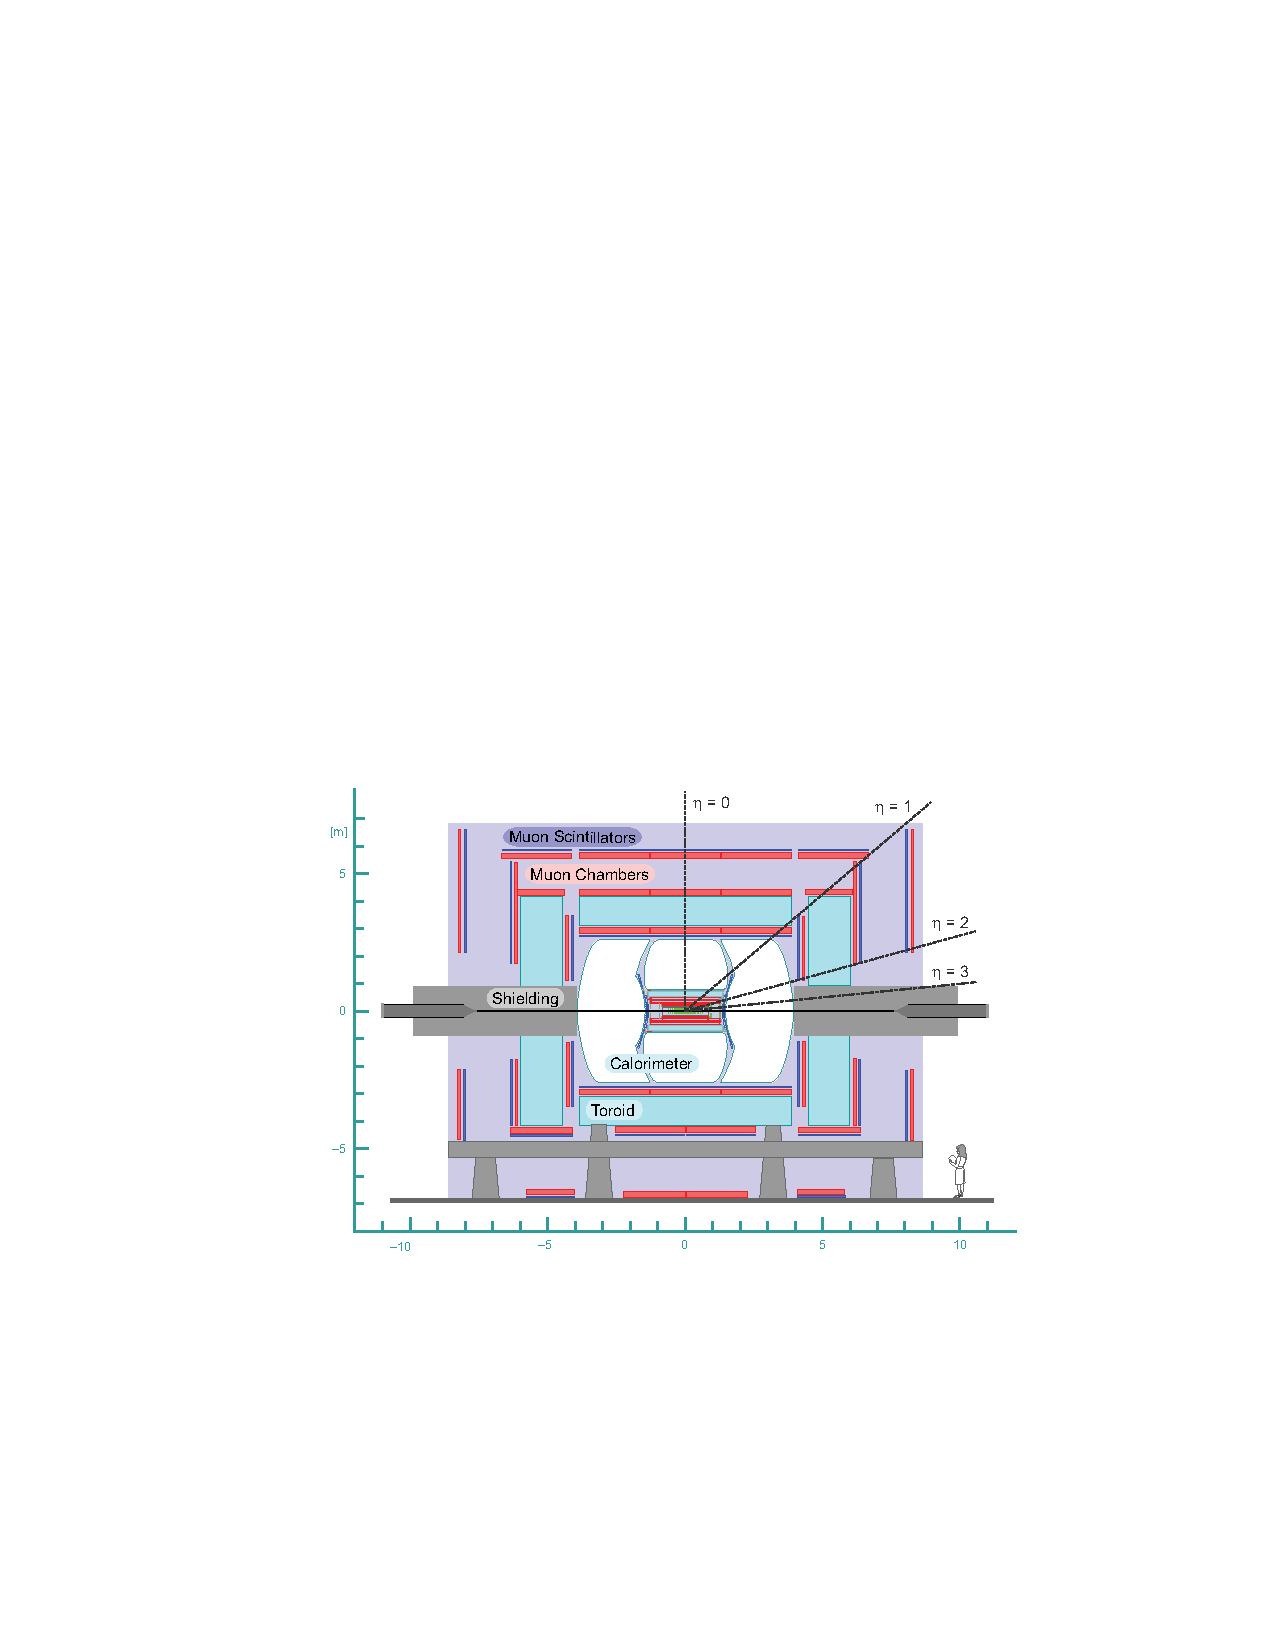
\includegraphics[width=0.45\textwidth]{./Images/01_dzero_wholedetector.pdf}};
%       \onslide<2->\zoombox[magnification=5,color code=lime]{0.86,0.35}
%     \end{tikzpicture}
%   \end{figure}
% \end{frame}  
